%% 1. DUAL-DISPLAY NOTES:
%\documentclass[hyperref={bookmarks=false}]{beamer}
%\usepackage{pgfpages}
%\setbeameroption{show notes on second screen=left}

% 2. NOTES ON SEPARATE SLIDES:
%\documentclass[xcolor=dvipsnames,9pt,show notes]{beamer}

% 3. NOTES ONLY:
%\documentclass[xcolor=dvipsnames,9pt,show only notes]{beamer}

% 4. HANDOUTS:
%\documentclass[xcolor=dvipsnames,9pt,handout,show notes]{beamer}

% 5. NO NOTES: ONLY ONE THAT BUILDS WITHOUT WARNINGS
\documentclass[xcolor=dvipsnames,9pt,hide notes,mathserif]{beamer}
%\setbeameroption{show only notes}
%\setbeameroption{show notes}
\usepackage{enumerate,amsmath,amssymb,fancyhdr,mathrsfs,amsthm,url,stmaryrd}
\usepackage{pgfpages}
\usepackage{listings}

%% For creating a handout:
%\pgfpagesuselayout{4 on 1}[border shrink=5mm]
%\mode<handout>{\setbeamercolor{background canvas}{bg=black!5}}

\setbeamerfont{structure}{family=\rmfamily,shape=\scshape} 
\usepackage{graphicx}
\usepackage{tikz}
\usepackage{scalefnt}
\usetikzlibrary{matrix,arrows}

\usepackage{mathrsfs,textcomp}
\setbeamertemplate{navigation symbols}{}
\usepackage{verbatim}
\usepackage[mathcal]{euscript}

\definecolor{Crimson}{rgb}{0.800,0.000,0.200}
\definecolor{darkred}{rgb}{0.5,0,0}
\newcommand{\Alert}[1]{\textcolor{darkred}{{\bf \emph{#1}}}}
\renewcommand{\alert}[1]{\textcolor{darkred}{\emph{#1}}}
\newcommand{\Eq}{\ensuremath{\operatorname{Eq}}}
\newcommand{\Con}{\ensuremath{\operatorname{Con}}}
\newcommand{\Sub}{\ensuremath{\operatorname{Sub}}}
\newcommand{\NSub}{\ensuremath{\operatorname{NSub}}}
\renewcommand{\phi}{\ensuremath{\operatorname{\varphi}}}
\renewcommand{\leq}{\ensuremath{\leqslant}}
\renewcommand{\nleq}{\ensuremath{\nleqslant}}
\renewcommand{\geq}{\ensuremath{\geqslant}}
\renewcommand{\gneq}{\ensuremath{\gneqslant}}
\renewcommand{\ngeq}{\ensuremath{\ngeqslant}}
\newcommand{\ssubnormal}{\ensuremath{\vartriangleleft}}
\newcommand{\subnormal}{\ensuremath{\trianglelefteqslant}}
\newcommand{\supnormal}{\ensuremath{\trianglerighteqslant}}
\newcommand{\notsubnormal}{\ensuremath{\ntrianglelefteqslant}}
\setbeamercolor{block title example}{fg=darkred,bg=white} %orange!20!black}

\usecolortheme[named=darkred]{structure} 
\setbeamertemplate{items}[ball] 
\setbeamertemplate{blocks}[rounded][shadow=true] 

\mode<presentation>{\usetheme{boxes}}

\usepackage[english]{babel}
\usepackage[latin1]{inputenc}
\usepackage{times}
\usepackage[T1]{fontenc}
% Or whatever. Note that the encoding and the font should match. If T1
% does not look nice, try deleting the line with the fontenc.

\title[Synchronizing Automata]{Dedekind's transposition principle\\
{\small and}\\
isotopic algebras with nonisomorphic\\ congruence lattices}
\author[William DeMeo]{William DeMeo\\
{\small \url{williamdemeo@gmail.com}}
}
\institute[\url{williamdemeo@gmail}]{{\small {\color{darkred}  University of South Carolina}}}

\date[AMS Sectional Meeting -- Boulder, CO]{
AMS Spring Western Sectional Meeting\\
University of Colorado, Boulder, CO \\[6pt]
April 13-14, 2013
}

\subject{Universal Algebra; Lattice Theory.}% (optional) inserted into PDF info catalog.

% TOC pops up at the beginning of each subsection:
\AtBeginSubsection[]{
  \begin{frame}<beamer>
    \frametitle{Outline}
    \tableofcontents[currentsection,currentsubsection]
  \end{frame}
}

\setbeamercovered{opaque}

%%%% INSERT MACROS %%%%
\newcommand{\bA}{\ensuremath{\mathbf{A}}}
\newcommand{\cA}{\ensuremath{\mathcal{A}}}
\newcommand{\fA}{\ensuremath{\mathfrak{A}}}
\newcommand{\sA}{\ensuremath{\mathscr{A}}}

\newcommand{\cB}{\ensuremath{\mathcal{B}}}
\newcommand{\bB}{\ensuremath{\mathbf{B}}}
\newcommand{\bBi}{\ensuremath{\mathbf{B}_i}}
\newcommand{\sB}{\ensuremath{\mathscr{B}}}
\newcommand{\fB}{\ensuremath{\mathfrak{B}}}

\newcommand{\bC}{\ensuremath{\mathbf{C}}}
\newcommand{\bF}{\ensuremath{\mathbf{F}}}
\newcommand{\sF}{\ensuremath{\mathcal{F}}}

\newcommand{\bL}{\ensuremath{\mathbf{L}}}

\newcommand{\lb}{\ensuremath{\llbracket}}
\newcommand{\rb}{\ensuremath{\rrbracket}}
\newcommand{\meet}{\ensuremath{\wedge}}
\newcommand{\join}{\ensuremath{\vee}}
\newcommand{\Meet}{\ensuremath{\bigwedge}}
\renewcommand{\Join}{\ensuremath{\bigvee}}

\newtheorem{prop}[theorem]{Proposition}
\newtheorem{assumption}[theorem]{Assumption}
\theoremstyle{definition}
\newtheorem{question}[theorem]{Question}
\newcounter{claim}
\newtheorem{claim}[claim]{Claim}
\newcounter{conjecture}
\newtheorem{conjecture}[conjecture]{Conjecture}
\newtheorem{case}{Case}
\theoremstyle{remark}
\newtheorem*{computations}{Computations}
\newtheorem*{remark}{Remark}
\newtheorem*{remarks}{Remarks}
\newtheorem*{notation}{Notation}
\numberwithin{theorem}{section}
\numberwithin{claim}{section}
\numberwithin{equation}{section}
\numberwithin{conjecture}{section}

\newcommand{\czerny}{\v{C}ern\'{y}}
\newcommand{\defn}[1]{\textcolor{darkred}{\textit{#1}}}
\newcommand{\IE}{{\small IE}}
\newcommand{\Op}{\ensuremath{\operatorname{Op}}}

\newcommand{\<}{\ensuremath{\langle}}
\renewcommand{\>}{\ensuremath{\rangle}}
\newcommand{\Clo}{\ensuremath{\mathrm{Clo}}}




%%%%%%%%%%%%  BEGIN DOCUMENT %%%%%%%%%%%%%%%

\begin{document}
\thicklines


%%% START HERE %%%
\frame[label=titlepage]{
  \titlepage
\vskip-3mm
  \begin{columns}
    \begin{column}{0.8\textwidth}
      \begin{center}
        {\small {\it These slides and other resources are available at}}\\[4pt]
 {\color{darkred}       \url{http://williamdemeo.wordpress.com}}
         \end{center}
       \end{column}
   \begin{column}{0.3\textwidth}
 \begin{tikzpicture}
            \node[opacity=0.9] (img2) at (2,-2){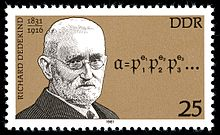
\includegraphics[height=18mm]{Dedekind-stamp}};
        \end{tikzpicture}
   \end{column}
    \end{columns}
}

\providecommand{\url}[1]{{#1}}
\providecommand{\urlprefix}{URL }


\section{Dedekind's Transposition Principle}
\newcommand\dotsize{.6pt}
%% \usebackgroundtemplate{%
%% \tikz\node[opacity=0.3] {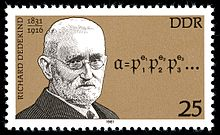
\includegraphics[height=\paperheight,widht=\paperwidth]{Dedekind-stamp}};}

%% \usebackgroundtemplate{%
%%   \vbox to \paperheight{\vfil\hbox to \paperwidth{\hfil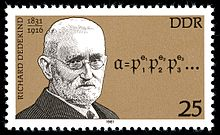
\includegraphics[width=1.5in]{Dedekind-stamp}\hfil}\vfil}
%% }

\begin{frame}[label=intro]{Dedekind's Transposition Principle}{for modular
    lattices}

  \begin{columns}
    \begin{column}{0.65\textwidth}
      {\bf Notation}

      \vskip2mm

      Let $\bL = \<L, \meet, \join\>$ be a lattice with $a \in L$.  

      \vskip2mm

      Let $\phi_a$ and $\psi_a$ be the \emph{perspectivity maps}
      \[
      \phi_a(x) = x\meet a \quad \text{ and }\quad 
      \psi_a(x) = x\join a
      \]
    For $x, y \in L$, let $\lb x, y \rb_L = \{ z\in L \mid x \leq z \leq
      y\}$.
    \end{column}

    \begin{column}{0.4\textwidth}
      \uncover<3->{
        {\scalefont{.9}
          \begin{tikzpicture}[scale=.4]

            \node (H) at (4,4) [draw,circle,inner sep=\dotsize] {}; \draw (H) node [right] {$b$};
            \node (U) at (-4,4) [draw,circle,inner sep=\dotsize] {}; \draw (U) node [left] {$a$};
            \node (U0) at (0,0) [draw,circle,inner sep=\dotsize] {}; 
            \draw (.7,-.5) node {$a\meet b$};
            \node (UH) at (0,8) [draw,circle,inner sep=\dotsize] {}; \draw (UH) node
                  [above] {$a\join b$};
                  \draw (U) to [out=-10,in=100] (U0) to [out=170,in=-80] (U)
                  (UH) to [out=-10,in=100] (H) to [out=170,in=-80] (UH);
                  \draw[dotted] 
                  (H) to [out=190,in=80] (U0) to [out=10,in=-100] (H)
                  (UH) to [out=190,in=80] (U) to [out=10,in=-100] (UH);

                  \shade[bottom color=darkred,top color=gray!-45] %            \fill[color=darkred] 
                  (U) to [out=-10,in=100] (U0) to [out=170,in=-80] (U);
                  \shade[bottom color=darkred,top color=gray!-45] 
                  %            \fill[color=darkred]
                  (UH) to [out=-10,in=100] (H) to [out=170,in=-80] (UH);
                  \node (V) at (-2.3,2.5) [fill,circle,inner sep=\dotsize] {}; \draw (V) node [left] {$x$};
                  \node (VH) at (1.7,6.5)[fill,circle,inner sep=\dotsize] {}; \draw (VH) node [right] {$\psi_b(x)$};
                  \node (X) at (2.5,5.3) [fill,circle,inner sep=\dotsize] {}; \draw (X) node [right] {$y$};
                  \node (UcapX) at (-1.5,1.3)[fill,circle,inner sep=\dotsize] {};  \draw (UcapX) node [left] {$\phi_a(y)$};
                  \draw[semithick,->] 
                  (V) to [out=65,in=-155] (VH);
                  \draw[semithick,->] 
                  (X) to [out=-155,in=65] (UcapX);
          \end{tikzpicture}
        }
      }
    \end{column}
  \end{columns}

  \vskip4mm


\uncover<2->{
\begin{columns}
    \begin{column}{0.75\textwidth}
  \begin{theorem}[Dedekind's Transposition Principle]
    $\bL$ is modular iff for all $a, b\in L$ the maps $\phi_a$ and $\psi_b$ are
    inverse lattice isomorphisms of $\lb a\meet b, a \rb$ and $\lb b, a\join b\rb$.

~
  \end{theorem}
   \end{column}
 
   \begin{column}{0.25\textwidth}

    \end{column}
\end{columns}
}

\end{frame}

\section{Another transposition principle}
\begin{frame}[label=intro]{Another transposition principle}
{for lattices of equivalence relations}
Let $X$ be a set and let $\Eq X$ be the lattice of equivalence relations on $X$.  

\vskip2mm

If $L$ is a sublattice of $\Eq X$ with $\eta,
\theta \in L$, then we define

\[
\lb \eta, \theta\rb_L = \{\gamma \in L \mid \eta \leq \gamma \leq \theta\}.
\]

\vskip2mm

\uncover<2->{
For $\beta \in \Eq X$, let $\lb \eta, \theta \rb_L^\beta$ be the set of
relations in $\lb \eta, \theta \rb_L$  that permute with
$\beta$,
\[
\lb \eta, \theta \rb_L^\beta = \{\gamma \in L \mid \eta \leq \gamma \leq
\theta \text{ and } \gamma \circ \beta = \beta \circ \gamma\}.
\]
}
\vskip-2mm
\uncover<3->{
\begin{columns}
    \begin{column}{0.7\textwidth}
\begin{lemma}
\label{lem:1}
Suppose $\alpha$ and $\beta$ are permuting relations in $L\leq \Eq X$.
\[\text{Then } \; \lb\beta, \alpha \join \beta\rb_L \cong \lb\alpha \meet \beta, \alpha\rb_L^\beta \leq 
\lb\alpha \meet \beta, \alpha\rb_L.
\]
\end{lemma}
    \end{column}
 
   \begin{column}{0.3\textwidth}
        {\scalefont{.9}
          \begin{tikzpicture}[scale=.35]

            \node (H) at (4,4) [draw,circle,inner sep=\dotsize] {}; \draw (H) node [right] {$\beta$};
            \node (U) at (-4,4) [draw,circle,inner sep=\dotsize] {}; \draw (U) node [left] {$\alpha$};
            \node (U0) at (0,0) [draw,circle,inner sep=\dotsize] {}; 
            \draw (1,-.5) node {$\alpha \meet \beta$};
            \node (UH) at (0,8) [draw,circle,inner sep=\dotsize] {}; \draw (UH) node
                  [above] {$\alpha \join \beta$};
                  \draw (U) to [out=-10,in=100] (U0) to [out=170,in=-80] (U)
                  (UH) to [out=-10,in=100] (H) to [out=170,in=-80] (UH);
                  \draw[dotted] 
                  (H) to [out=190,in=80] (U0) to [out=10,in=-100] (H)
                  (UH) to [out=190,in=80] (U) to [out=10,in=-100] (UH);

                  %\shade[bottom color=darkred,top color=gray!-45] %            
                  \fill[color=darkred] 
                  (U) to [out=-10,in=100] (U0) to [out=170,in=-80] (U);
                  \shade[bottom color=darkred,top color=gray!-45] 
                  %            \fill[color=darkred]
                  (UH) to [out=-10,in=100] (H) to [out=170,in=-80] (UH);
                  \node (V) at (-2.5,2.7) [fill,circle,inner sep=\dotsize] {}; \draw (V) node [left] {$x$};
                  \node (VH) at (2,6.75)[fill,circle,inner sep=\dotsize] {};
                  \draw (3,7.2) node {$x \circ \beta$};
                  \node (X) at (2.5,5.3) [fill,circle,inner sep=\dotsize] {}; \draw (X) node [right] {$y$};
                  \node (UcapX) at (-1.78,1.2)[fill,circle,inner sep=\dotsize] {};
                  \draw (-2.6,.4) node {$y \meet \alpha$};
                  \draw[semithick,->] 
                  (V) to [out=65,in=-155] (VH);
                  \draw[semithick,->] 
                  (X) to [out=-155,in=65] (UcapX);
          \end{tikzpicture}
      }

    \end{column}
\end{columns}
}

\end{frame}


\begin{frame}[label=intro]{Dedekind's Rule}
\note{
  The lemma states that the sublattice $\lb\beta, \alpha \join \beta\rb_L$ is isomorphic to the 
lattice, $\lb\alpha \meet \beta, \alpha\rb_L^\beta$, of relations in $L$ that are below
$\alpha$, above $\alpha \meet \beta$, and permute with $\beta$; moreover, $\lb\alpha \meet \beta,
\alpha\rb_L^\beta$ is a sublattice of
$\lb\alpha \meet \beta, \alpha\rb_L$.
}
The proof requires the following version of \emph{Dedekind's Rule:}
\note{In the group theory setting, the well known Dedekind's
  Rule states that if $A, B, C$ are subgroups of a group,
  and $A\leq B$, then we have the following identity of sets: $A(B\cap C) = B
  \cap AC$.}
\begin{lemma}
\label{lem:dedekind}
Suppose $\alpha, \beta, \gamma \in L \leq \Eq X$ and $\alpha
\leq \beta$.
\vskip2mm
Then the following identities of subsets of $X^2$ hold:
\begin{equation*}
  \label{eq:1}
  \alpha \circ (\beta \cap \gamma) = \beta \cap (\alpha \circ \gamma)
\end{equation*}
\begin{equation*}
  \label{eq:2}
  (\beta \cap \gamma) \circ \alpha = \beta \cap (\gamma \circ \alpha)
\end{equation*}
\end{lemma}

\end{frame}



\section{Isotopy}

\begin{frame}[label=intro]{Isotopy}{basic definitions}
Let $\bA$, $\bB$, $\bC$ be algebras of the same type.


\vskip2mm

$\bA$ and $\bB$ are \alert{isotopic over} $\bC$, denoted $\bA\sim_{\bC}\bB$,
if there is an isomorphism 
\[
\phi: \bA \times \bC \stackrel{\cong}{\longrightarrow} \bB \times \bC \quad
\text{ that leaves the second coordinate fixed }
\]
\[
\text{ i.e. } \; (\forall a\in A)\,(\forall c\in C) \quad \phi(a,c) = (\phi_1(a,c),c)
\]

\vskip2mm
\uncover<2->{
  We say that $\bA$ and $\bB$ are \alert{isotopic}, denoted $\bA\sim \bB$, if
  $\bA\sim_{\bC}\bB$ for some $\bC$.  
  \vskip2mm
}
\alt<2>{It is easy to verify that $\sim$ is an equivalence relation.
}{
  \onslide<3->{
    If $\bA\sim_{\bC}\bB$ and $\Con (\bA \times \bC)$ happens to
    be modular, then we write}
}
\uncover<3->{
$\bA \sim^{\mathrm{mod}}_{\bC} \bB$ and say that
$\bA$ and $\bB$ are \alert{modular isotopic over} $\bC$.
\vskip2mm
}
\onslide<4->{
We call $\bA$ and $\bB$ \alert{modular isotopic in one step},  denoted 
$\bA \sim^{\mathrm{mod}}_1 \bB$,
if they are modular isotopic over some $\bC$.
\vskip2mm
}
\onslide<5->{
We call $\bA$ and $\bB$ are \alert{modular isotopic}, denoted 
$\bA \sim^{\mathrm{mod}} \bB$, if $(\bA, \bB)$ is in the transitive
closure of $\sim^{\mathrm{mod}}_1$.
}

\end{frame}



\begin{frame}[label=intro]{Isotopy}{modular case}
%A well known 
%\vskip2mm
%~ \hskip 2cm 
{\bf Lemma 11.}\hskip2mm If $\bA \sim^{\mathrm{mod}} \bB$ then $\Con \bA \cong \Con \bB$.

\vskip2mm

The proof is a nice/easy application of Dedekind's Transposition Principle.  

\vskip2mm
\uncover<2->{
Could we use the same strategy with the non-modular version of the transposition principle to show that 
$\bA\sim\bB$ implies $\Con \bA \cong \Con \bB$?
}
\vskip2mm

\uncover<3->{As you have guessed, the answer is no!

\vskip2mm
The perspectivity map that is so useful
  when $\Con (\bA\times \bC)$ is modular can fail \emph{miserably} in the non-modular
  case...
\uncover<4->{ 
\emph{even when} $\bA \cong \bB$! } }

\vskip2mm
\uncover<5->{But this only shows that the same argument doesn't work...}

\end{frame}

\begin{frame}[label=intro]{Counterexamples}
  We describe a class of examples in which $\bA\sim \bB$ and $\Con \bA
  \ncong \Con \bB$. 

  \vskip2mm
  The examples show that congruence lattices of
  isotopic algebras can differ arbitrarily in size.

  \vskip2mm
  \uncover<2->{
    For any group $G$, let $\Sub(G)$ denote the lattice of subgroups of $G$.
  }
  \vskip2mm
  \uncover<3->{
    A group $G$ is called a \alert{Dedekind group} if every subgroup of $G$ is
    normal.
    \note{a \emph{non-Dedekind group} is one with a non-trivial non-normal subgroup.}
  }
  \note{of course this requires $G$ be nonabelian, but that is not
    sufficient.  For example, the eight element quaternion group 
    is a Dedekind group.}

  \vskip2mm
  \uncover<4->{
    Let $S$ be any group and let $D$ denote the \emph{diagonal subgroup} of 
    $S\times S$,
\[D = \{(x,x) \mid x\in S\}\]
  }

  \uncover<4->{
    The interval $\lb D, S\times S\rb \leq \Sub(S\times S)$ 
      is described by the following
    }
    \vskip2mm
    \uncover<4->{
      \begin{lemma}
        \label{lem:1}
        The filter above the diagonal subgroup of $S\times S$ %in the subgroup lattice of $S\times S$
        is isomorphic to the lattice of normal subgroups of $S$. 

~
    \end{lemma}
    }


\end{frame}


\section{Example}

\begin{frame}[label=example]{The example}

Let $S$ be a group, and 
let $G = S_1 \times S_2$, where
$S_1 \cong S_2 \cong S$. 

\vskip2mm
Let $D = \{(x_1,x_2)\in G \mid x_1 = x_2\}, \quad T_1 = S_1 \times \<1\>, \quad T_2 = \<1\>\times S_2$.
\vskip2mm

\vskip2mm
\uncover<2->{
Then $D \cong T_1 \cong T_2$, and these are pair-wise compliments:
\[
\<T_1, T_2\> = \<T_1,D\> = \<D, T_2\> = G
\]
\[
T_1\cap D = D\cap T_2 = T_1 \cap T_2 =
\<(1,1)\>
\]
}

\uncover<3->{
Let $\bA = \< G/T_1, G^{\bA}\> =$ the algebra with universe the left
cosets of $T_1$ in $G$, and basic operations the left multiplications by elements
of $G$. 
\vskip2mm
For each $g\in G$ the operation $g^{\bA} \in G^{\bA}$ is defined by
\[
g^{\bA}(xT_1) = 
(gx)T_1 \qquad ( xT_1 \in G/T_1 ).
\]
Define the algebra $\bC = \< G/T_2, G^{\bC}\>$ similarly.  
}
\end{frame}


\begin{frame}[label=example]{The example}
The algebra $\bB$ will have universe $B = G/D$, but we
define the action of $G$ on $B$ with a twist.
\vskip2mm
\uncover<2->{
For each $g = (g_1, g_2) \in G$,
for each $(x_1, x_2)D \in G/D$, define
\[
g^{\bB}((x_1,x_2)D) =  (g_2x_1, g_1 x_2)D.
\]
Let $\bB = \< G/D, G^{\bB}\>$, where $G^{\bB} =  \{g^{\bB} \mid g\in G\}$.
}
\vskip2mm
\uncover<3->{
Consider the binary relation 
$\phi \subseteq (A \times C) \times (B \times C)$ that associates
to each ordered pair 
\[((x_1,x_2)T_1, (y_1,y_2)T_2) \in A \times C\]
 the pair 
\[((x_2, y_1)D, (y_1,y_2)T_2) \in B \times C\]
}

\uncover<4->{
It is easy to verify that this relation is a function, and in fact 
\[
\phi \colon \bA \times \bC \rightarrow \bB \times \bC \; \text{ is an
  isomorphism.}
\]
}
\uncover<5->{
Since $\phi$ leaves second coordinates fixed,
$\bA\sim_{\bC}\bB$.  
}
\end{frame}


\section{Conclusion}
\begin{frame}[label=conclusion]{Conclusion}
Compare $\Con \bA$ and $\Con \bB$.
\vskip2mm
\uncover<2->{
$\Con \bA \cong \lb T_1, G\rb \leq \Sub(G)$, so $\Con \bA \cong \Sub(S)$.
%(see Lemma 4.20 of ALVi).
}
\vskip2mm
\uncover<3->{
$\Con \bB$ is isomorphic to the lattice of normal subgroups
of $S$.
}
\uncover<4->{
\[
\Con \bB \cong\NSub(S) \leq \Sub(S) \cong  \Con \bA
\] 
So, if $S$ is any non-Dedekind group, $\Con \bB \ncong \Con \bA$.
}
\vskip2mm
\uncover<5->{If $S$ is a nonabelian simple group, then $\Con \bB \cong
  \mathbf{2}$, while
$\Con \bA \cong \Sub(S)$ can be arbitrarily large.}

\end{frame}
\end{document}
